\documentclass[sigconf,nonacm]{acmart}

\usepackage{booktabs}
\usepackage{algorithm}
\usepackage{algpseudocode}

\settopmatter{printacmref=false}
\renewcommand\footnotetextcopyrightpermission[1]{}
\pagestyle{plain}

\newcommand{\Dt}{\Delta_t}
\newcommand{\ind}[1]{\mathbb{1}[#1]}

\begin{document}

\title{Preserving Diversity in Classifier-Free Guidance}

\author{Austin Zhao}
\authornote{Worked on interventions.}
\affiliation{%
  \institution{Cornell University}
  \city{New York}
  \state{NY}
  \country{USA}}
\email{az392@cornell.edu}

\author{Xinqi Yue}
\authornote{Worked on literature review, metrics, and baselines.}
\affiliation{%
  \institution{Cornell University}
  \city{New York}
  \state{NY}
  \country{USA}}
\email{xy549@cornell.edu}

\author{Edmond Kong}
\authornotemark[1]
\affiliation{%
  \institution{Cornell University}
  \city{New York}
  \state{NY}
  \country{USA}}
\email{eck67@cornell.edu}

\renewcommand{\shortauthors}{Zhao, Yue, and Kong}

\begin{abstract}
Classifier-free guidance (CFG) improves the fidelity and class consistency of diffusion samples, but at strong guidance scales it collapses within-class diversity: samples of the same class converge to similar layouts, poses and appearances. We study where and how this diversity is lost in Scalable Interpolant Transformers (SiT) on class-conditional ImageNet $256\times256$. Tracking the guidance vector across seeds, we find that during roughly the first 30\% of sampling it is largely shared by all samples of a class, and that guidance applied only in this early window reproduces essentially the full loss of layout diversity caused by guidance at $w=4$, along with most of the drop in effective rank in the later transformer blocks. Building on this, we compare interventions that weaken guidance only during the early window: scalar damping, score damping in a per-class shared subspace, low-frequency damping, damping of the class embedding (condition damping) and of block activations (feature damping), a delayed guidance interval, and a \emph{shuffled push} that rotates the shared guidance component differently for each sample instead of removing it. Score damping fully restores layout diversity while keeping 97\% of the fidelity gained by guidance, but recovers little semantic diversity; condition damping recovers far more semantic diversity at a substantial cost in fidelity, and no guidance start time matches score damping on both axes. The shuffled push recovers more layout and semantic diversity than score damping at the same measured fidelity, although visual inspection reveals color defects that our classifier-based fidelity measure does not capture.
\end{abstract}

\keywords{diffusion models, classifier-free guidance, sample diversity, diffusion transformers}

\maketitle

%% ===================================================================
\section{Introduction}
\label{sec:intro}

Diffusion models have achieved impressive results in image generation, and Classifier-Free Guidance (CFG) is widely used to improve the quality and class consistency of generated images by combining conditional and unconditional model predictions during sampling~\cite{ho2022cfg}. However, strong guidance introduces a trade-off between sample quality and diversity~\cite{ho2022cfg}. Although increasing the guidance scale can improve fidelity to the target class, it can also reduce within-class diversity, making the generated images share similar layouts, poses and appearances. Our research therefore asks: where and how is diversity lost during the sampling process, and can it be recovered without sacrificing generation quality?

Our investigation builds on several studies of diffusion models and guidance methods. Peebles and Xie~\cite{peebles2023dit} introduced the Diffusion Transformer (DiT), which uses transformer architectures for image generation. Ma et al.~\cite{ma2024sit} extended this with Scalable Interpolant Transformers (SiT), which place the same architecture in an interpolant framework that unifies flow and diffusion models. We use these architectures as the foundation of our experiments. More recent work has explored ways to mitigate diversity loss. For example, CADS adds noise to the conditioning signal during sampling~\cite{sadat2024cads}, while Guidance Interval applies guidance only within a selected time interval~\cite{kynkaanniemi2024interval}. Adaptive Projected Guidance (APG) modifies the guidance direction to reduce unwanted effects at high guidance scales~\cite{sadat2025apg}, and Frequency-Decoupled Guidance (FDG) applies different guidance strengths to low- and high-frequency components, using weaker guidance on the low frequencies that control global structure~\cite{sadat2025fdg}. In addition, Jin et al.~\cite{jin2026stagewise} analyze the stage-wise effects of CFG and show how guidance affects diversity at different stages of sampling.

In this work, we first locate where diversity is lost by tracking the within-class spread of the guidance signal and of the model's internal activations over sampling time. We find that layout diversity is lost within roughly the first 30\% of sampling, when guidance pushes all samples of a class along a shared direction. Based on this, we propose damping methods that weaken only this early, shared component of the guidance, compare them with existing approaches such as delayed guidance intervals, and test whether the shared push can be redirected per sample rather than removed.

%% ===================================================================
\section{Methods}
\label{sec:methods}

\subsection{Data and Experimental Setup}
\label{sec:data}

We use ImageNet-1K at $256\times256$ resolution, the standard class-conditional benchmark of DiT and SiT, which has 1{,}000 classes. We do not train any model. We use the pretrained SiT-L/2 for the analysis and plan to use the official SiT-XL/2 for the full comparison of methods. Both models operate in the $32\times32\times4$ latent space of the Stable Diffusion VAE. We sample with the Euler method on a 50-point time grid (49 Euler steps), with time running from $t=0$ (pure noise) to $t=1$ (data).

All results in this report use SiT-L/2 with guidance scale $w=4$ on eight ImageNet classes (golden retriever, otter, lesser panda, geyser, macaw, valley, balloon and arctic fox). Methods that require calibration estimate their subspaces on seeds 0--15, and all methods are evaluated on the held-out seeds 16--31 (128 images per condition). Every condition uses identical initial noise and two network evaluations per step. For the distribution-level metrics, we plan to compare generated images with the standard ImageNet $256\times256$ reference batch of ADM~\cite{dhariwal2021beat}.

\subsection{Evaluation Metrics}
\label{sec:metrics}

Table~\ref{tab:metrics} lists the metrics we use. Within-class diversity metrics need no real images. They are computed within each class across seeds and then averaged over classes, and they are used for the preliminary results in this report: \emph{layout diversity} is the spread $V_{\text{low}}$ of the low-pass final latents, and \emph{semantic diversity} is the mean pairwise cosine distance $1-\mathrm{MSS}$ of DINOv2 and of CLIP features. Distribution-level metrics need about 50{,}000 samples and real-image statistics, so they are planned for the full evaluation. Until then, class fidelity serves as a quality proxy.

\begin{table*}[t]
  \caption{Evaluation metrics. $\uparrow$ higher is better, $\downarrow$ lower is better. Y: used in this report; P: planned.}
  \label{tab:metrics}
  \small
  \begin{tabular}{@{}p{0.14\textwidth}p{0.5\textwidth}ccc@{}}
    \toprule
    Metric & Definition & Better & SiT-L/2 analysis & SiT-XL/2 baselines \\
    \midrule
    \multicolumn{5}{@{}l}{\emph{Within-class diversity}} \\
    Vendi~\cite{friedman2023vendi} & $\exp\!\big(-\sum_k \mu_k \log \mu_k\big)$, where $\mu_k$ is the $k$-th eigenvalue of the DINOv2 cosine-similarity matrix divided by the number of samples $n$; the effective number of distinct samples & $\uparrow$ & -- & Y \\
    MSS & Mean pairwise cosine similarity of DINOv2 and CLIP features & $\downarrow$ & Y\textsuperscript{a} & Y \\
    Spread $V$ & $1 - \lVert \bar{x} \rVert^2 / \operatorname{mean}_i \lVert x_i \rVert^2$: scale-free spread around the class mean, on $\hat{x}_t$ over sampling time and on low-pass final latents ($V_{\text{low}}$, layout) & $\uparrow$ & Y & Y \\
    \midrule
    \multicolumn{5}{@{}l}{\emph{Quality}} \\
    Class fidelity & Pretrained ImageNet classifier's confidence in the target class & $\uparrow$ & Y & Y \\
    FID~\cite{heusel2017fid} & Fr\'echet distance between Inception-v3 feature distributions of real and generated images & $\downarrow$ & P & P \\
    IS & Inception Score: confident and varied class predictions & $\uparrow$ & P & P \\
    Precision / Recall~\cite{kynkaanniemi2019precision} & Share of generated samples in the real-image manifold (fidelity) / share of real images in the generated manifold (coverage) & $\uparrow$ & P & P \\
    FD\textsubscript{DINOv2}~\cite{stein2023exposing} & Fr\'echet distance on DINOv2 features & $\downarrow$ & P & P \\
    \bottomrule
    \multicolumn{5}{@{}l}{\footnotesize \textsuperscript{a}Reported as the mean pairwise cosine distance, $1-\mathrm{MSS}$.}
  \end{tabular}
\end{table*}

\paragraph{Diversity recovery.}
To compare interventions, we express each measure relative to the unguided ($w=1$) and fully guided ($w=4$) references. For each diversity measure $D \in \{D_{\text{layout}}, D_{\text{DINO}}, D_{\text{CLIP}}\}$, the recovery of a condition is the fraction of the diversity lost at $w=4$ that it regains:
\begin{equation}
  R_D = \frac{D - D^{(w=4)}}{D^{(w=1)} - D^{(w=4)}} .
  \label{eq:recovery}
\end{equation}
$R_D = 0$ means no diversity is recovered, $R_D = 1$ means diversity is restored to the unguided level, and $R_D > 1$ means the condition is more diverse than $w=1$.

\paragraph{Fidelity retention.}
As a proxy for class fidelity, we classify each decoded image with an ImageNet classifier (ViT-B/16, pretrained on ImageNet-21k and fine-tuned on ImageNet-1k) and record the softmax probability of the intended class, averaged over seeds and classes:
\begin{equation}
  P = \frac{1}{|\mathcal{C}|\, n} \sum_{c \in \mathcal{C}} \sum_{s=1}^{n}
  \operatorname{softmax}\big(g(I^{(s,c)})\big)_c ,
  \label{eq:fidelity}
\end{equation}
where $g$ outputs the classifier's logits and $I^{(s,c)}$ is the decoded image for seed $s$ and class $c$. Fidelity retention is the fraction of the fidelity gained by guidance that a condition keeps:
\begin{equation}
  F = \frac{P - P^{(w=1)}}{P^{(w=4)} - P^{(w=1)}} .
  \label{eq:retention}
\end{equation}
$F = 1$ means fidelity is as high as plain guidance, and $F = 0$ means it has fallen to the unguided level. An ideal intervention has $R_D$ and $F$ both close to $1$.

\paragraph{Uncertainty.}
We resample the seeds 1000 times, using the same seed indices for every condition including both references, and recompute each ratio. Intervals are the 2.5th and 97.5th percentiles. Repeated seeds are removed from each resample, because identical copies would count as shared variation and artificially lower diversity.

\subsection{Windowed Guidance}
\label{sec:windowed}

Classifier-free guidance takes a linear combination of the conditional and unconditional predictions~\cite{ho2022cfg}:
\begin{equation}
  \tilde{\epsilon}_\theta(x_t, c) = \epsilon_\theta(x_t) + w\big(\epsilon_\theta(x_t, c) - \epsilon_\theta(x_t)\big),
  \label{eq:cfg}
\end{equation}
where the guidance strength $w$ sets the magnitude of the \emph{guidance vector} $\Delta = \epsilon_\theta(x_t, c) - \epsilon_\theta(x_t)$:
\begin{equation}
  \tilde{\epsilon}_\theta(x_t, c) = \epsilon_\theta(x_t) + w\Delta .
  \label{eq:cfg-delta}
\end{equation}
Intuitively, $\Delta$ is the offset of the prediction for samples of class $c$ from the prediction for all plausible samples; that is, the ``unique'' direction that class $c$ takes in its denoising trajectory.

SiT predicts a velocity rather than noise, and guidance is applied to it in the same way. Writing $v_\theta(x_t, t, c)$ and $v_\theta(x_t, t, \varnothing)$ for the conditional and unconditional velocities and $\Dt = v_\theta(x_t, t, c) - v_\theta(x_t, t, \varnothing)$, the guided velocity is
\begin{equation}
  f_t = v_\theta(x_t, t, \varnothing) + w\,\Dt = v_\theta(x_t, t, c) + (w-1)\,\Dt ,
  \label{eq:cfg-velocity}
\end{equation}
so that $(w-1)\Dt$ is the \emph{excess guidance} beyond the conditional prediction. SiT guides only the first three of the four latent channels, so $\Dt \in \mathbb{R}^D$ with $D = 3 \times 32 \times 32$. Based on our observation of where diversity is lost (Section~\ref{sec:res-shared}), we let the guidance depend on the timestep $t$, which we call \emph{windowed guidance}. All of the methods below modify guidance only during an early window $t < \tau$, with $\tau = 0.3$ unless stated otherwise, and use full guidance $w$ afterwards.

\subsection{Scalar Damping and Guidance Interval}
\label{sec:scalar}

Increasing the guidance strength pushes the prediction more strongly in the direction of class $c$; conversely, decreasing it weakens this effect. We call a decrease in $w$ during the early window \emph{scalar damping}:
\begin{equation}
  w_t = \begin{cases} 1 + (w-1)(1-\lambda), & t < \tau \\ w, & t \ge \tau \end{cases}
  \label{eq:scalar}
\end{equation}
where $\lambda$ is the damping strength. Setting $w_t = 1$ ($\lambda = 1$) removes classifier-free guidance during the window and keeps only the conditional prediction.

\paragraph{Guidance interval.}
Scalar damping at $\lambda = 1$ is a step schedule that follows the conditional prediction before $\tau$ and applies full guidance after it. This is the guidance-interval method of Kynk\"a\"anniemi et al.~\cite{kynkaanniemi2024interval}, which disables guidance at the noisiest steps. Since the damping methods below restrict guidance both in time ($t < \tau$) and in direction, we use this schedule to isolate the effect of timing alone: we vary the switch-on time $\tau \in \{0.1, 0.2, 0.3, 0.4, 0.5\}$ and compare each setting with score damping ($\lambda = 1$, $\tau = 0.3$).

\subsection{Score Damping}
\label{sec:score}

Scalar damping damps every direction of $\Delta$ equally. However, not all directions of $\Delta$ vary equally within a class. We therefore remove only the components of $\Delta$ along the top $k$ shared directions of the class ($k=3$).

\paragraph{Shared guidance subspace.}
On a set of calibration seeds $\mathcal{S}$ (disjoint from the evaluation seeds), we average $\Delta$ over seeds so that seed-specific components cancel and we are left with shared class components:
\begin{equation}
  \bar{\Delta}_t^{(c)} = \frac{1}{|\mathcal{S}|} \sum_{s \in \mathcal{S}} \Delta_t^{(s,c)} .
  \label{eq:mean-delta}
\end{equation}
We stack these means over the early steps $\mathcal{T} = \{t : t < \tau\}$ as the rows of
\begin{equation}
  M_c = \begin{bmatrix}
    \big(\bar{\Delta}_t^{(c)}\big)^{\!\top}_{w=1,\; t \in \mathcal{T}} \\[2pt]
    \big(\bar{\Delta}_t^{(c)}\big)^{\!\top}_{w=4,\; t \in \mathcal{T}}
  \end{bmatrix}
  \in \mathbb{R}^{2|\mathcal{T}| \times D},
  \label{eq:stack}
\end{equation}
and take its (uncentered) singular value decomposition $M_c = U \Sigma V^{\top}$. Let $B_c \in \mathbb{R}^{k \times D}$ hold the first $k$ right singular vectors as orthonormal rows. The projector onto class $c$'s shared guidance subspace is
\begin{equation}
  P_c = B_c^{\top} B_c \in \mathbb{R}^{D \times D} .
  \label{eq:projector}
\end{equation}

\paragraph{Damped guidance.}
At each step, the component of the sample's own $\Dt$ inside this subspace is damped by strength $\lambda$ during the early window:
\begin{equation}
  \tilde{\Delta}_t = \big(I - \lambda\, \ind{t < \tau}\, P_c\big)\, \Dt ,
  \label{eq:score-damp}
\end{equation}
and only the excess guidance uses the damped vector:
\begin{equation}
  \tilde{f}_t = v_\theta(x_t, t, c) + (w-1)\,\tilde{\Delta}_t .
  \label{eq:score-guided}
\end{equation}
Equivalently, the effective guidance weight is $w$ on the orthogonal complement of the subspace and
\begin{equation}
  w_{\text{eff}} = 1 + (w-1)(1-\lambda)
  \label{eq:weff}
\end{equation}
inside it, matching scalar damping (Eq.~\eqref{eq:scalar}) within the subspace. At $\lambda = 1$ the shared directions receive no guidance beyond the conditional prediction ($w_{\text{eff}} = 1$), while $\lambda > 1$ pushes against them. As a control for whether class-specific directions matter, the \emph{wrong-class} condition applies score damping with the subspace of a different class.

\subsection{Shuffled Push}
\label{sec:shuffled}

Score damping removes excess guidance inside the shared subspace. The shuffled push tests whether diversity is lost because of the shared push itself, or because every sample of a class is pushed in the same direction. It keeps the component at full strength but rotates it within the subspace, differently for each sample:
\begin{equation}
  a_t = B_c\,\Dt, \qquad
  \tilde{\Delta}_t = \begin{cases} \Dt - \lambda\,B_c^{\top}\big(a_t - R_{s,c}\,a_t\big), & t < \tau \\ \Dt, & t \ge \tau \end{cases}
  \label{eq:shuffled}
\end{equation}
with $\tilde{f}_t$ as in Eq.~\eqref{eq:score-guided}. Here $a_t \in \mathbb{R}^k$ is the shared push in subspace coordinates and $R_{s,c} \in \mathbb{R}^{k \times k}$ rotates it; $B_c^{\top}$ maps the difference back to the full guidance vector, so at $\lambda = 1$ the shared push is replaced by its rotated copy. Setting $R = 0$ recovers score damping (Section~\ref{sec:score}), which subtracts the shared push and adds nothing back, and $R = I_k$ gives plain guidance. The shuffled push draws $R_{s,c}$ as a uniformly random rotation in $SO(k)$, once per seed $s$ and class $c$, held fixed over all steps and drawn independently of the initial noise.

Since $\lVert R_{s,c}\,a_t \rVert = \lVert a_t \rVert$ and $(I - P_c)\Dt$ is unchanged, at $\lambda = 1$ each sample keeps a shared-subspace push as strong as under plain guidance, but in its own direction, turned by $90^\circ$ on average. The two methods thus differ only in $R$, isolating the effect of rotating rather than removing the shared push. Like APG~\cite{sadat2025apg}, this changes the guidance direction rather than its magnitude. Algorithm~\ref{alg:shuffled} summarizes the sampler. We compare the shuffled push with score damping at $\lambda \in \{0.5, 1\}$, with condition damping ($\lambda = 0.5$, Section~\ref{sec:condition}) as a reference.

\begin{algorithm}[t]
  \caption{Euler sampling with the shuffled push}
  \label{alg:shuffled}
  \begin{algorithmic}[1]
    \State $x \gets x_0 \sim \mathcal{N}(0, I)$ from seed $s$; \quad $R \gets \textsc{RandomRotation}(s, c)$
    \For{$i = 0, \dots, K-1$}
      \State $t \gets i/K$; \quad $v_c \gets v_\theta(x, t, c)$; \quad $\Delta \gets v_c - v_\theta(x, t, \varnothing)$
      \If{$t < \tau$}
        \State $a \gets B_c \Delta$; \quad $\Delta \gets \Delta - \lambda B_c^{\top}(a - R a)$
      \EndIf
      \State $x \gets x + \big(v_c + (w-1)\Delta\big)/K$
    \EndFor
    \State \Return $x$
  \end{algorithmic}
\end{algorithm}

\subsection{Frequency Damping}
\label{sec:frequency}

Score damping requires calibration seeds to estimate each class's shared subspace. Early guidance, however, mostly sets global layout, which lives at low spatial frequencies. Frequency damping therefore replaces the learned projector with a fixed low-pass filter that needs no calibration and is the same for every class.

\paragraph{Low-pass projector.}
Let $P_{\text{low}} \in \mathbb{R}^{D \times D}$ be the orthogonal projector that keeps, in each guided channel of $\Dt$, only the spatial frequencies $\mathbf{k}$ with $\lVert \mathbf{k} \rVert_2 \le \kappa$ cycles per image (we use $\kappa = 4$). Appendix~\ref{app:lowpass} gives its construction from the 2D discrete Fourier transform.

\paragraph{Damped guidance.}
As with score damping, the sample's own $\Dt$ loses a fraction $\lambda$ of its low-frequency component during the early window:
\begin{equation}
  \tilde{\Delta}_t = \big(I - \lambda\, \ind{t < \tau}\, P_{\text{low}}\big)\, \Dt ,
  \qquad
  \tilde{f}_t = v_\theta(x_t, t, c) + (w-1)\,\tilde{\Delta}_t .
  \label{eq:freq-damp}
\end{equation}
The effective guidance weight is $1 + (w-1)(1-\lambda)$ for frequencies with $\lVert \mathbf{k} \rVert_2 \le \kappa$ and $w$ for all higher frequencies, so at $\lambda = 1$ the coarse layout receives no guidance beyond the conditional prediction while fine detail stays fully guided.

\subsection{Condition Damping}
\label{sec:condition}

Score and frequency damping edit the guidance vector after the network has produced it, so the network's internal computation at that step is unchanged. The condition vector, which encodes the class $c$, is instead passed in directly at every transformer block. \emph{Condition damping} weakens the class label at the network's input, so the damping propagates through every transformer block. Like frequency damping, it needs no calibration.

\paragraph{Class conditioning in SiT.}
SiT maps each class label $y$, and a null label $\varnothing$ used for classifier-free guidance, to a learned embedding $e_y \in \mathbb{R}^{1024}$. This embedding is added to the timestep embedding, and the sum conditions every block through adaptive layer normalization (adaLN), which sets the scale and shift of each layer. We write $v_\theta(x_t, t, e)$ for the velocity prediction given conditioning embedding $e$, so that $\Dt = v_\theta(x_t, t, e_c) - v_\theta(x_t, t, e_\varnothing)$.

\paragraph{Damped embedding.}
During the early window, the conditional pass receives an embedding interpolated from the null embedding toward the class embedding:
\begin{equation}
  e'_c = e_\varnothing + \alpha_t\,(e_c - e_\varnothing),
  \qquad
  \alpha_t = 1 - \lambda\, \ind{t < \tau}\, \frac{w-1}{w} .
  \label{eq:cond-embed}
\end{equation}
The unconditional pass is unchanged, and standard classifier-free guidance is applied with the original weight $w$:
\begin{equation}
  \tilde{\Delta}_t = v_\theta(x_t, t, e'_c) - v_\theta(x_t, t, e_\varnothing),
  \qquad
  \tilde{f}_t = v_\theta(x_t, t, e_\varnothing) + w\,\tilde{\Delta}_t .
  \label{eq:cond-guided}
\end{equation}

\paragraph{Choice of $\alpha$.}
The scale $\alpha_t$ is chosen so that, to first order in the embedding, the effective guidance weight during the window is $w_{\text{eff}} = w\,\alpha_t = 1 + (w-1)(1-\lambda)$, matching scalar, score and frequency damping (Appendix~\ref{app:cond}). At $\lambda = 1$, $\alpha = 1/w$ and the early steps receive approximately no guidance beyond the conditional prediction. Unlike the other methods, this damping is not restricted to a subspace: it weakens the entire class signal, and it does so through the network rather than on its output.

\paragraph{Differences from output-space damping.}
Because condition damping changes the conditional prediction itself, it also affects the fourth latent channel, which SiT's \texttt{forward\_with\_cfg} leaves unguided and which scalar, score and frequency damping therefore leave untouched. Because the network is nonlinear in $e$, the relation $w_{\text{eff}} = w\alpha_t$ holds only to first order, so the realized guidance strength at a given $\lambda$ can differ from that of the other methods.

\subsection{Feature Damping}
\label{sec:feature}

While the preceding methods act on the whole model input or denoising step, \emph{feature damping} is more targeted: it removes only the shared class component of the activations, and only in the later blocks $\mathcal{B}$ (blocks 13--23), where cross-seed effective rank falls most under strong guidance (Section~\ref{sec:res-rank}).

\paragraph{Internal class signal.}
Let $h_{b,t}(x_t, e) \in \mathbb{R}^{N \times C}$ be the output of transformer block $b$, with $N$ tokens and $C$ channels, and let $\bar{h}_{b,t} = \frac{1}{N} \sum_{i=1}^{N} h_{b,t}[i] \in \mathbb{R}^{C}$ be its token-pooled mean. For seed $s$ and class $c$, the internal class signal at block $b$ is the difference between the conditional and unconditional passes on the same $x_t$:
\begin{equation}
  \delta_{b,t}^{(s,c)} = \bar{h}_{b,t}\big(x_t^{(s,c)}, e_c\big) - \bar{h}_{b,t}\big(x_t^{(s,c)}, e_\varnothing\big)
  \in \mathbb{R}^{C} .
  \label{eq:feat-signal}
\end{equation}

\paragraph{Shared feature subspace.}
Exactly as for score damping (Eqs.~\eqref{eq:mean-delta}--\eqref{eq:projector}), we average $\delta_{b,t}^{(s,c)}$ over the calibration seeds, stack the means over the early steps and keep the top $k$ right singular vectors, giving one projector $Q_{b,c} \in \mathbb{R}^{C \times C}$ per block and class (Appendix~\ref{app:feat}).

\paragraph{Damped activations.}
During the early window, after each block $b \in \mathcal{B}$, the conditional pass's activations are shifted, by the same amount at every token, to remove part of the shared class signal measured on the current sample:
\begin{equation}
  \tilde{h}_{b,t}[i] = h_{b,t}[i] - \lambda\, \ind{t < \tau}\, \frac{w-1}{w}\,
  Q_{b,c}\, \delta_{b,t},
  \qquad i = 1, \dots, N .
  \label{eq:feat-damp}
\end{equation}
The unconditional pass is unchanged, and $\tilde{h}_{b,t}$ is passed on to block $b+1$. The final output is guided as usual, $\tilde{f}_t = v_\theta(x_t, t, e_\varnothing) + w\,\tilde{\Delta}_t$, where $\tilde{\Delta}_t$ is computed from the modified conditional pass.

The factor $(w-1)/w$ is chosen, as in condition damping, so that at $\lambda = 1$ the targeted component receives approximately no guidance beyond the conditional prediction (Appendix~\ref{app:feat}).

%% ===================================================================
\section{Results}
\label{sec:results}

\subsection{Shared Guidance over the Denoising Trajectory}
\label{sec:res-shared}

Diversity decreases when the randomness introduced by the seed does not manifest in the resulting image. To investigate where in the denoising trajectory diversity is lost, we measure, averaged over the eight classes, the mean pairwise cosine similarity of $\Delta$ and the shared proportion of $\Delta$, the conditional velocity $v_\theta(x_t, t, c)$ and the unconditional velocity $v_\theta(x_t, t, \varnothing)$ (Figure~\ref{fig:shared}).

\paragraph{Shared proportion.}
For a quantity $v^{(s)} \in \mathbb{R}^{D}$ measured on seeds $s = 1, \dots, n$ of the same class at the same step, let $\bar{v} = \frac{1}{n} \sum_{s=1}^{n} v^{(s)}$ be its cross-seed mean. The shared proportion is
\begin{equation}
  S(v) = \frac{\lVert \bar{v} \rVert_2^2}{\frac{1}{n} \sum_{s=1}^{n} \lVert v^{(s)} \rVert_2^2} .
  \label{eq:shared}
\end{equation}

We find that $\Delta$ is mostly shared among denoising trajectories of the same class before $t = 0.3$ (Figure~\ref{fig:shared}). Therefore, in our windowed guidance approaches, we limit our interventions to $t < 0.3$.

\begin{figure}[t]
  \centering
  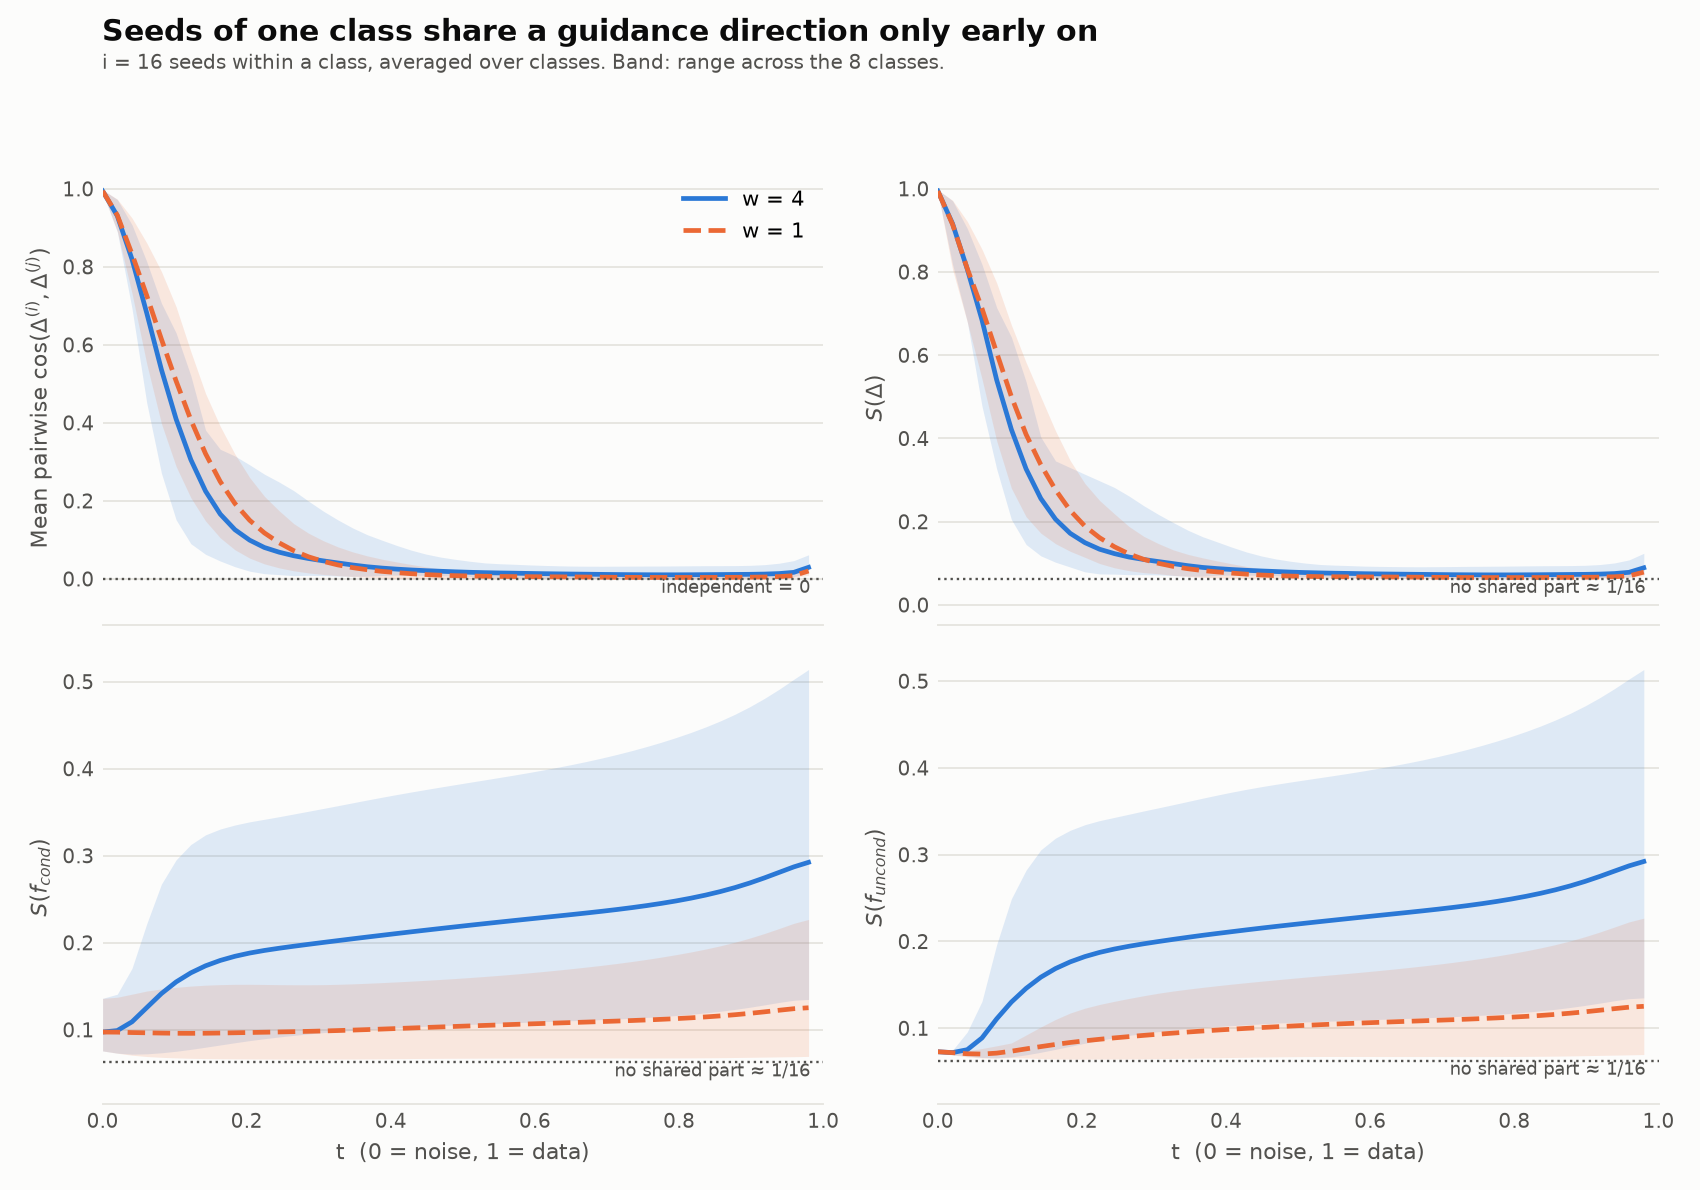
\includegraphics[width=\linewidth]{figures/shared_guidance.png}
  \caption{Within-class agreement over timestep $t$, averaged over eight classes. Top left: mean pairwise cosine similarity of $\Delta$ across seeds. Top right: shared proportion of $\Delta$. Bottom left: shared proportion of the conditional velocity $v_\theta(x_t, t, c)$ ($f_{\text{cond}}$ in the plot). Bottom right: shared proportion of the unconditional velocity $v_\theta(x_t, t, \varnothing)$ ($f_{\text{uncond}}$).}
  \Description{Four line plots over sampling time showing that the guidance vector is highly shared across seeds of a class before t equals 0.3 and much less shared afterwards.}
  \label{fig:shared}
\end{figure}

\subsection{Effective Rank of Transformer Blocks over the Denoising Trajectory}
\label{sec:res-rank}

To understand where in the model guidance reduces diversity, we look at the effective rank of the model's activations at each block, pooled over the height and width dimensions. Effective rank measures how many independent directions the activations of different seeds actually vary along. If guidance pushes every seed's activations toward the same few directions, the samples can only differ in a few ways, and effective rank falls.

Increased guidance ($w = 4$) decreases the effective rank in roughly blocks 12--23 and increases it in blocks 1--11 (Figure~\ref{fig:rank-w4}). Importantly, mid-to-late transformer blocks contain the most ``semantic'' representations of the model's output~\cite{yu2025repa}. We therefore hypothesize that an intervention on these blocks would be most effective.

\begin{figure}[t]
  \centering
  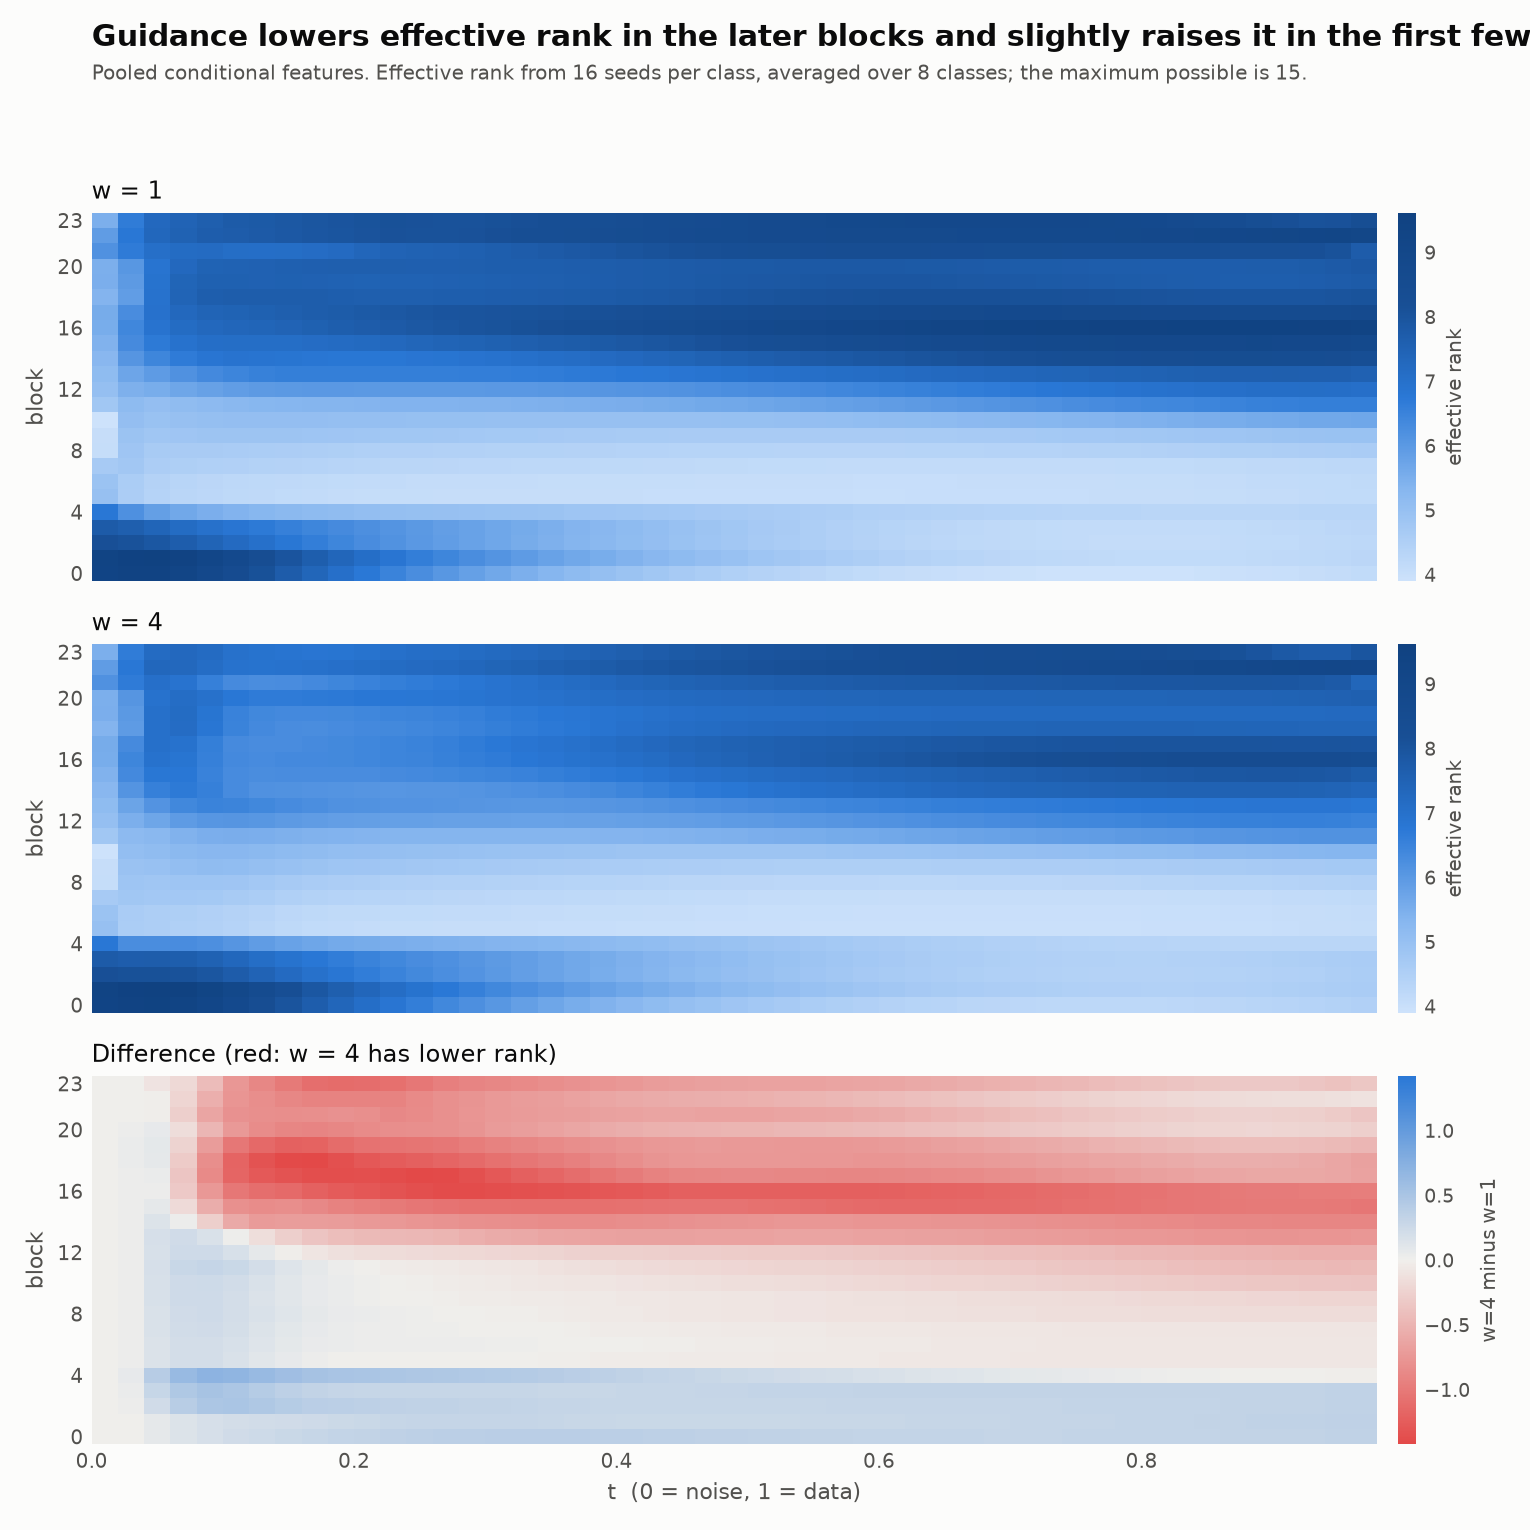
\includegraphics[width=0.9\linewidth]{figures/effective_rank_w4.png}
  \caption{Difference in effective rank of pooled activations at each transformer block over timestep $t$, between $w = 4$ and $w = 1$. Red: lower rank at $w = 4$; blue: higher rank at $w = 4$.}
  \Description{Heatmap of transformer block versus sampling time. Later blocks are red, indicating lower effective rank under strong guidance, and earlier blocks are blue.}
  \label{fig:rank-w4}
\end{figure}

\subsection{Early Versus Late Guidance}
\label{sec:res-early-late}

To understand the effect of early and late guidance on diversity, we compare applying guidance only in an early interval $t < 0.3$ with applying it only in a late interval $t \ge 0.3$ (Table~\ref{tab:early-late}). Early guidance alone reproduces nearly the full reduction in effective rank and in final latent diversity caused by $w = 4$, while late guidance alone reproduces only about a third of the rank reduction and almost none of the latent diversity loss. However, the loss of semantic diversity, measured in DINOv2 and CLIP embeddings, is reproduced to a similar degree by either interval (0.58--0.72). This suggests that interventions that act only on the guided output at the early steps, without changing the model's internal computation, tend to affect finer structure rather than meaningfully change the semantics of the generated image.

\begin{table}[t]
  \caption{Diversity loss reproduced by applying guidance only early or only late, as a share of the full effect of $w = 4$.}
  \label{tab:early-late}
  \small
  \begin{tabular}{@{}lcc@{}}
    \toprule
    Measure & Early ($t < 0.3$) & Late ($t \ge 0.3$) \\
    \midrule
    Effective rank, blocks 13--23 & 0.97 & 0.37 \\
    Final latent diversity (cosine sim.) & 1.03 & 0.03 \\
    Final DINOv2 diversity & 0.69 & 0.69 \\
    Final CLIP diversity & 0.72 & 0.58 \\
    \bottomrule
  \end{tabular}
\end{table}

\subsection{Comparison of Interventions}
\label{sec:res-interventions}

For each intervention, run only within the window $t < 0.3$, we evaluate layout, DINOv2 and CLIP recovery (Eq.~\eqref{eq:recovery}) and fidelity retention (Eq.~\eqref{eq:retention}) of the final samples (Table~\ref{tab:interventions}).

Score damping fully recovers layout diversity while largely maintaining fidelity. Condition damping at $\lambda = 1$ recovers far more layout and semantic (DINOv2, CLIP) diversity, at the cost of fidelity retention. Score damping therefore most likely increases diversity in low-frequency structure that is secondary to the image's main subject, which limits its semantic recovery. Condition damping, on the other hand, pushes the model to generate an image more ``general'' than class $c$, which may produce more unrealistic or ambiguous images. Feature damping recovers little diversity of any kind, and the wrong-class control recovers far less layout diversity than score damping, indicating that the class-specific subspace matters.

\begin{table}[t]
  \caption{Diversity recovery $R_D$ and fidelity retention $F$ for each intervention, applied for $t < 0.3$ (SiT-L/2, $w = 4$, seeds 16--31).}
  \label{tab:interventions}
  \small
  \begin{tabular}{@{}lcccc@{}}
    \toprule
    & \multicolumn{3}{c}{Recovery $R_D$} & \\
    \cmidrule(lr){2-4}
    Condition & Layout & DINOv2 & CLIP & Fidelity $F$ \\
    \midrule
    Scalar, $\lambda = 1$ & 0.95 & 0.28 & 0.38 & 0.84 \\
    Score, $\lambda = 1$ & 1.01 & 0.10 & 0.17 & 0.97 \\
    Frequency, $\lambda = 1$ & 0.92 & 0.20 & 0.29 & 0.89 \\
    Condition, $\lambda = 0.5$ & 0.57 & 0.17 & 0.25 & 0.96 \\
    Condition, $\lambda = 1$ & 1.29 & 0.44 & 0.70 & 0.71 \\
    Feature, $\lambda = 1$ & 0.09 & 0.05 & 0.10 & 0.97 \\
    Wrong class, $\lambda = 1$ & 0.20 & $-0.01$ & 0.00 & 0.99 \\
    \bottomrule
  \end{tabular}
\end{table}

\subsection{Mechanistic Study of Interventions}
\label{sec:res-mech}

To understand how the interventions affect the model internally, we plot the effective rank of pooled activations by transformer block over time and compare it to the $w = 4$ case (Figure~\ref{fig:rank-interventions}). Condition damping raises the effective rank of the more ``semantic'' later blocks more strongly than score damping, and the increase is largest when score and condition damping are combined. The effects persist after the intervention window $t < 0.3$, although more weakly.

\begin{figure*}[t]
  \centering
  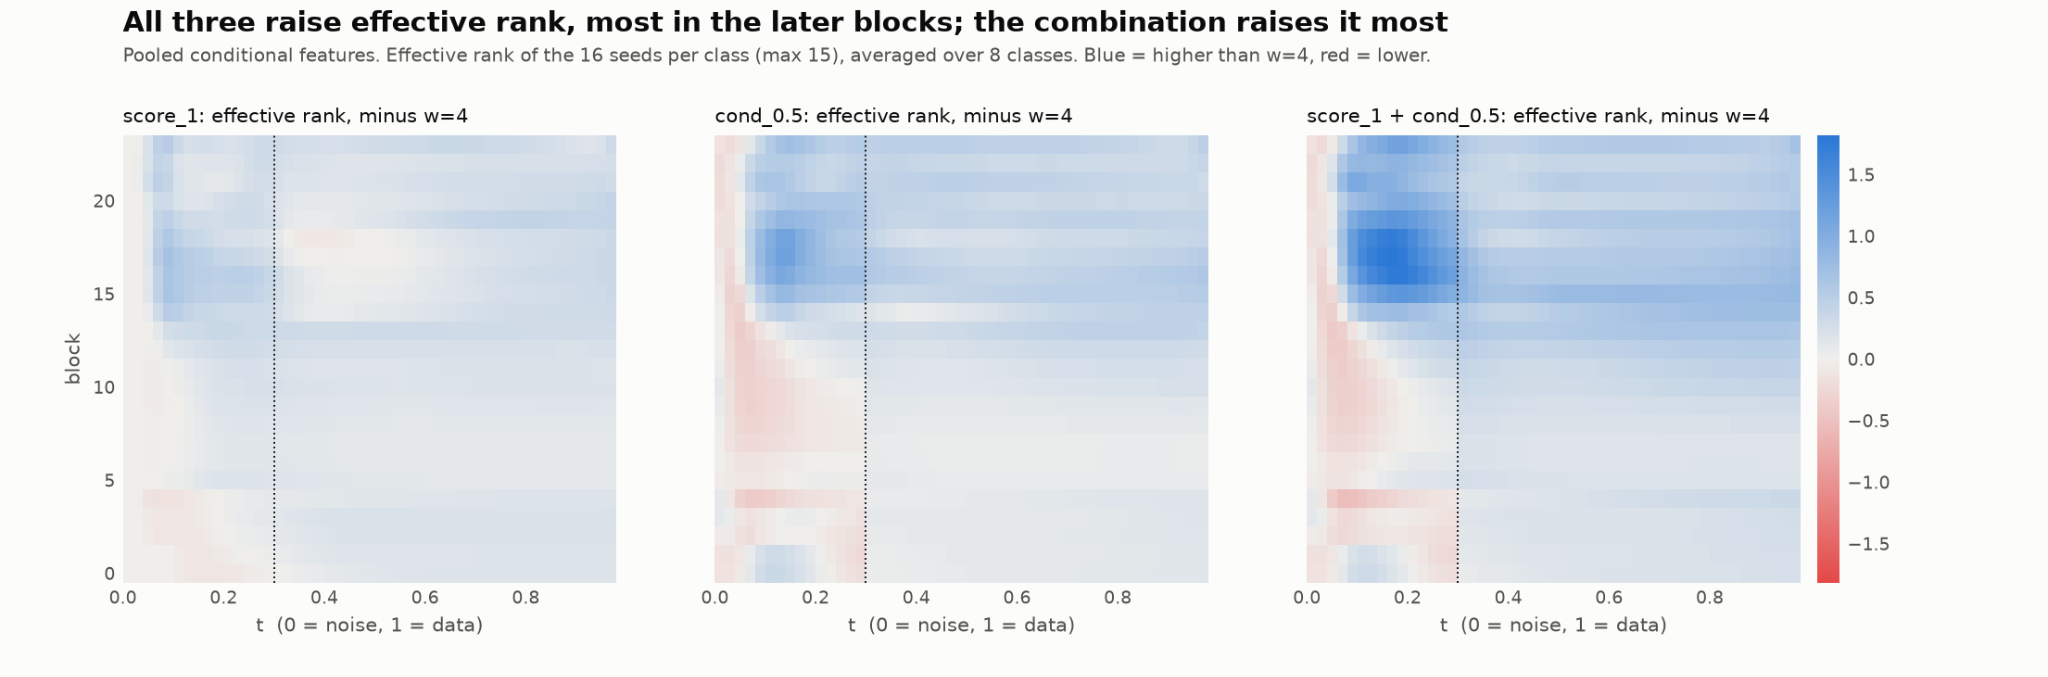
\includegraphics[width=\textwidth]{figures/effective_rank_interventions.png}
  \caption{Difference in effective rank of pooled activations at each transformer block over timestep $t$, between each intervention and $w = 4$. Red: lower rank at $w = 4$; blue: higher rank at $w = 4$ (compared to the intervention).}
  \Description{Heatmaps of transformer block versus sampling time for each intervention, showing that condition damping raises effective rank in later blocks more than score damping.}
  \label{fig:rank-interventions}
\end{figure*}

\subsection{Delaying the Start of Guidance}
\label{sec:res-interval}

Table~\ref{tab:interval} and Figure~\ref{fig:recovery} show that delaying guidance offers a trade-off: later start times recover more diversity but retain less fidelity. Layout recovery jumps from 0.69 at $\tau = 0.1$ to 0.88 at $\tau = 0.2$, then plateaus between 0.95 and 0.99 for $\tau \ge 0.3$. The $\tau = 0.3$ setting is identical to scalar damping with $\lambda = 1$ (Table~\ref{tab:interventions}). No start time matches score damping's layout recovery at comparable fidelity, so the timing of guidance alone is not enough to preserve diversity. Late starts do recover semantic diversity, but at a steep cost: at $\tau = 0.5$ only 63\% of the fidelity gained by guidance is retained.

\begin{table}[t]
  \caption{Diversity recovery and fidelity retention for the guidance interval with switch-on time $\tau$, compared with score damping.}
  \label{tab:interval}
  \small
  \begin{tabular}{@{}lcccc@{}}
    \toprule
    & \multicolumn{3}{c}{Recovery $R_D$} & \\
    \cmidrule(lr){2-4}
    Condition & Layout & DINOv2 & CLIP & Fidelity $F$ \\
    \midrule
    Interval, $\tau = 0.1$ & 0.69 & 0.08 & 0.11 & 0.96 \\
    Interval, $\tau = 0.2$ & 0.88 & 0.15 & 0.23 & 0.93 \\
    Interval, $\tau = 0.3$ & 0.95 & 0.28 & 0.38 & 0.84 \\
    Interval, $\tau = 0.4$ & 0.98 & 0.38 & 0.49 & 0.78 \\
    Interval, $\tau = 0.5$ & 0.99 & 0.55 & 0.64 & 0.63 \\
    \midrule
    Score damping, $\lambda = 1$ & 1.01 & 0.10 & 0.17 & 0.97 \\
    \bottomrule
  \end{tabular}
\end{table}

\begin{figure*}[t]
  \centering
  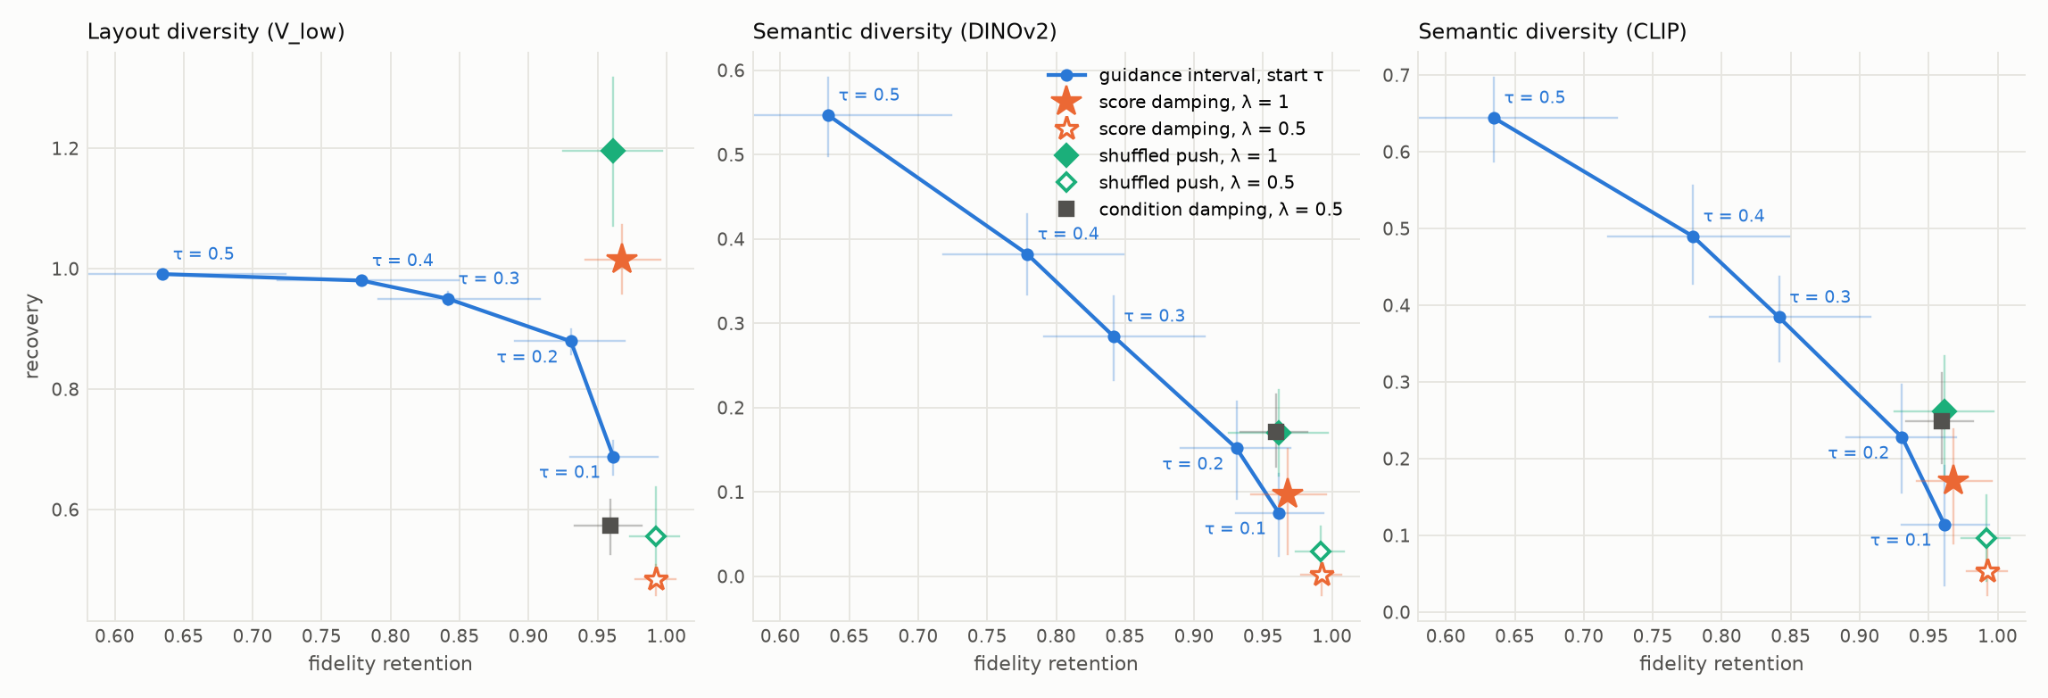
\includegraphics[width=\textwidth]{figures/recovery_vs_fidelity.png}
  \caption{Diversity recovery against fidelity retention for the guidance interval (varying $\tau$), score damping, the shuffled push and condition damping, on seeds 16--31. Left: layout diversity ($V_{\text{low}}$). Middle: semantic diversity (DINOv2). Right: semantic diversity (CLIP). Error bars are 95\% bootstrap intervals.}
  \Description{Three scatter plots of recovery versus fidelity retention. The guidance-interval curve trades fidelity for diversity; the shuffled push at lambda 1 lies above score damping at similar fidelity.}
  \label{fig:recovery}
\end{figure*}

\subsection{Shuffled Push}
\label{sec:res-shuffled}

At $\lambda = 1$ the shuffled push beats score damping on layout ($+0.18$), DINOv2 ($+0.07$) and CLIP ($+0.09$) recovery, with no significant difference in fidelity retention (Table~\ref{tab:shuffled}, Figure~\ref{fig:recovery}). At $\lambda = 0.5$ the gains are smaller but in the same direction.

\begin{table}[t]
  \caption{Diversity recovery and fidelity retention for the shuffled push and score damping.}
  \label{tab:shuffled}
  \small
  \begin{tabular}{@{}lcccc@{}}
    \toprule
    & \multicolumn{3}{c}{Recovery $R_D$} & \\
    \cmidrule(lr){2-4}
    Condition & Layout & DINOv2 & CLIP & Fidelity $F$ \\
    \midrule
    Score damping, $\lambda = 0.5$ & 0.48 & 0.00 & 0.05 & 0.99 \\
    Shuffled push, $\lambda = 0.5$ & 0.55 & 0.03 & 0.10 & 0.99 \\
    Score damping, $\lambda = 1$ & 1.01 & 0.10 & 0.17 & 0.97 \\
    Shuffled push, $\lambda = 1$ & 1.20 & 0.17 & 0.26 & 0.96 \\
    \bottomrule
  \end{tabular}
\end{table}

However, Figures~\ref{fig:seed19} and~\ref{fig:seed16} show fidelity differences that our metrics do not capture. The shuffled push strongly recolored 25 of 128 images, whereas score damping recolored only 2 and $w = 1$ recolored 6. For example, the shuffled push produced a pink geyser (Figure~\ref{fig:seed19}) and an underexposed dog (Figure~\ref{fig:seed16}). This is an early indicator of a limitation of our evaluation: fidelity is measured as classifier confidence, which misses color defects that are obvious to the human eye.

\begin{figure}[t]
  \centering
  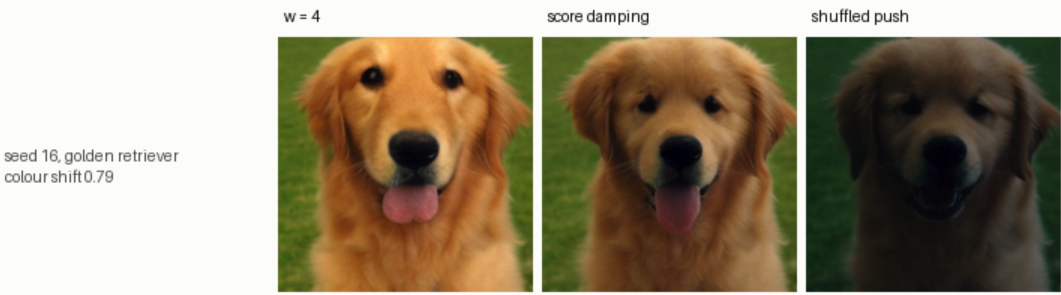
\includegraphics[width=\linewidth]{figures/seed16_color_shift.png}
  \caption{Color shift after the shuffled push: seed 16, golden retriever, under $w = 4$, score damping and the shuffled push ($\lambda = 1$).}
  \Description{Three images of a golden retriever. The shuffled-push image is much darker than the other two.}
  \label{fig:seed16}
\end{figure}

\begin{figure*}[t]
  \centering
  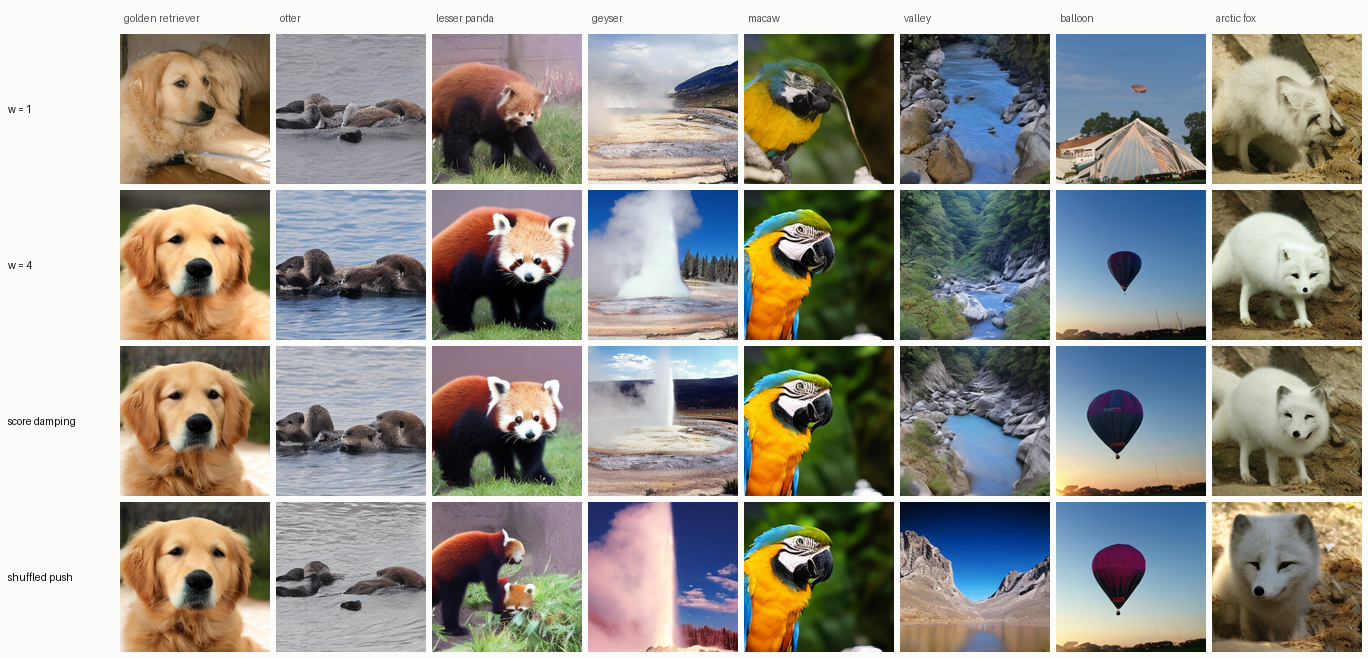
\includegraphics[width=\textwidth]{figures/seed19_grid.png}
  \caption{Samples for seed 19 across the eight classes under $w = 1$, $w = 4$, score damping and the shuffled push ($\lambda = 1$).}
  \Description{A grid of images with four rows (w equals 1, w equals 4, score damping, shuffled push) and eight class columns. The shuffled-push geyser is tinted pink.}
  \label{fig:seed19}
\end{figure*}


%% ===================================================================
\section*{AI Disclosure}

Claude Code and Gemini generated all code and graphs, which were manually verified.

\bibliographystyle{ACM-Reference-Format}
\bibliography{references}

\appendix

\section{Construction of the Low-Pass Projector}
\label{app:lowpass}

Each guided channel of $\Dt$ is an $l \times l$ grid, where $l$ is the width of the latent image. Let $F \in \mathbb{C}^{l^2 \times l^2}$ be the unitary 2D discrete Fourier transform on one channel, with integer frequencies $\mathbf{k} = (k_1, k_2)$, $k_i \in \{-\frac{l}{2}, \dots, \frac{l}{2}-1\}$ (cycles per image). For a cutoff $\kappa$, define the radial mask
\begin{equation}
  m(\mathbf{k}) = \ind{\lVert \mathbf{k} \rVert_2 \le \kappa}
  \label{eq:mask}
\end{equation}
and the per-channel filter
\begin{equation}
  L = F^{-1} \operatorname{diag}(m)\, F \in \mathbb{R}^{l^2 \times l^2} .
  \label{eq:lowpass}
\end{equation}
Because $m$ takes values in $\{0, 1\}$ and is symmetric under $\mathbf{k} \mapsto -\mathbf{k}$, $L$ is real, symmetric and idempotent, so it is an orthogonal projector onto the low-frequency subspace. Applying it to each guided channel separately gives
\begin{equation}
  P_{\text{low}} = I_3 \otimes L \in \mathbb{R}^{D \times D} .
  \label{eq:plow}
\end{equation}

\section{Effective Guidance Weight of Condition Damping}
\label{app:cond}

Linearizing the network in its conditioning embedding around $e_\varnothing$,
\begin{equation}
  \tilde{\Delta}_t \approx J_t\,\alpha_t\,(e_c - e_\varnothing) \approx \alpha_t\,\Dt,
  \qquad
  J_t = \frac{\partial v_\theta(x_t, t, e)}{\partial e}\bigg|_{e = e_\varnothing},
  \label{eq:linearize}
\end{equation}
so the effective guidance weight is
\begin{equation}
  w_{\text{eff}} = w\,\alpha_t = 1 + (w-1)(1-\lambda)
  \label{eq:cond-weff}
\end{equation}
for $t < \tau$, matching the effective weight of scalar, score and frequency damping. At $\lambda = 1$, $\alpha = 1/w$ and the early steps receive approximately no guidance beyond the conditional prediction.

\section{Feature Damping Details}
\label{app:feat}

\paragraph{Shared feature subspace.}
Exactly as for score damping, we average over the calibration seeds $\mathcal{S}$,
\begin{equation}
  \bar{\delta}_{b,t}^{(c)} = \frac{1}{|\mathcal{S}|} \sum_{s \in \mathcal{S}} \delta_{b,t}^{(s,c)} ,
  \label{eq:feat-mean}
\end{equation}
stack these means over the early steps $t \in \mathcal{T}$ into $M_{b,c} \in \mathbb{R}^{2|\mathcal{T}| \times C}$, and take its uncentered SVD. The first $k$ right singular vectors form the rows of $U_{b,c} \in \mathbb{R}^{k \times C}$, giving one projector per block and class:
\begin{equation}
  Q_{b,c} = U_{b,c}^{\top} U_{b,c} \in \mathbb{R}^{C \times C} .
  \label{eq:feat-proj}
\end{equation}

\paragraph{Choice of the factor $(w-1)/w$.}
The edit changes the conditional branch, whose difference from the unconditional branch is multiplied by $w$ in guidance. Removing a fraction $(w-1)/w$ of the targeted component leaves $w\big(1 - \tfrac{w-1}{w}\big) = 1$ times that component at $\lambda = 1$, to first order. This is the same target as condition damping, and matches the effective weight $1 + (w-1)(1-\lambda)$ of the other methods inside the subspace.

\end{document}
